\section{Die Vorreiterrolle Englands}
\label{sec:vorr-gb}
\index{Großbritannien!wirtschaftlich}
\index{Industrialisierung!Großbritannien}

\begin{figure}
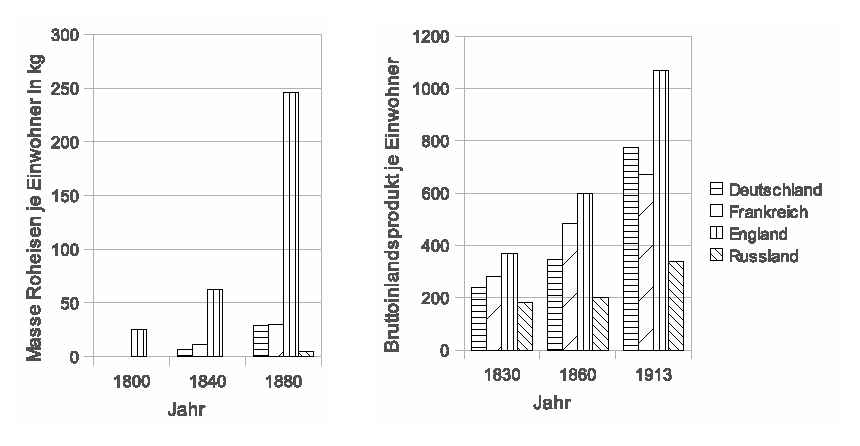
\includegraphics[width=\textwidth]{vorr-gb-diag.eps}
\caption{Roheisenproduktion und Bruttoinlandsprodukt europäischer
Staaten}
\label{pic:vorr-gb-diag}
\end{figure}

\paragraph{Wie Abbildung \ref{pic:vorr-gb-diag} zeigt,} hat
Großbritannien den wirtschaftlichen Entwicklungsprozeß deutlich eher
und mit deutlich höherer Intensität begonnen als andere europäische
Staaten. Es gilt also herauszufinden, wie es zu dieser rasanten
Entwicklung kam.\\

\begin{aufgabe}
Begründen Sie die Vorreiterrolle Englands anhand der besonderen
Voraussetzungen, die dieses Land im Industrialisierungsprozeß
hatte!\footnote{Dazu ist der Inhalt von Abbildung
\ref{pic:vorr-gb-diag} hinreichend}
\end{aufgabe} 

\subsection{Innenpolitische Entwicklung}
\index{Großbritannien!innenpolitisch}

Die \dat{Große Revolution von 1640 bis 1688}
\index{Großbritannien!Große Revolution} \index{Glorious Revolution}
hatte der mittelalterlich"=feudalen Epoche in England ein Ende gesetzt.
Die neue Verfassung sah zensusgebundenes Wahlrecht und
Parlamentssitzvergabe vor und ermöglichte so der \beg{gentry}, den
alten Feudaladel zu verdrängen und ihre fortschrittlichen
wirtschaftlichen Interessen durchzusetzen.

Außerdem sorgte die scharfe Abgrenzung zwischen den Schichten --
Unter-, Oberschicht, Bedienstete etc. -- für eine klare Regelung der
gesellschaftlichen und sozialen Verhältnisse. 


\subsection{Außenpolitische Entwicklung}
\index{Großbritannien!außenpolitisch}

\paragraph{\nam{Henry \Rm{7}} (1486\,--\,1509)} England beginnt eine lange
Tradition der internationalen Seefahrt.

\paragraph{\nam{Elisabeth \Rm{1}} (1558\,--\,1603)} Die englische Flotte
erringt den \dat{Sieg gegen die spanische Armada} und wird so zur
Seemacht. -- Außenhandel und Piraterie weiten sich aus.

\paragraph{\nam{James \Rm{1}} (1603\,--\,1625)} erwirbt 13 Kolonien als
Rohstoffquellen für England und legt so den Grundstein für eine
gezielte Kolonialpolitik.

\paragraph{\Nam{Cromwell, Oliver}{Oliver Cromwell}
(1599\,--\,1658)} England sichert seine Vormachtstellung auf See durch
Siege gegen Holland und Spanien und erwirbt weitere Kolonien, wie zum
Beispiel Jamaika.

\paragraph{\nam{Charles \Rm{2}} (1660\,--\,1685)} Der Krieg gegen
Holland bringt neue Kolonien -- Neuholland und Neuamsterdam.

\paragraph{1714\,--\,1815} Großbritannien erweitert im \dat{War of
Jenkins' Ear 1739\,--\,1742} seinen Kolonialbesitz, erwirbt durch das
Wegfallen Frankreichs als Konkurrenten durch den \dat{Siebenjährigen
Krieg 1756\,--\,1763} Kanada und steigt so endgültig zur Weltmacht
auf.\\

Großbritannien hatte also vor allem durch Handel und Seefahrt einen
gewaltigen Vorrat an Macht, Geld, Rohstoffen, Arbeitern und
Absatzmärkten gewonnen. Dieser bildete die Grundlage für den rasanten
Industrialisierungsprozeß. Abbildung \ref{pic:vorr-gb-gr} bietet
nochmals einen Überblick.

\begin{figure}
\centering
%\begin{sideways}
%\input{vorr-gb-gr.eepic}
%\end{sideways}
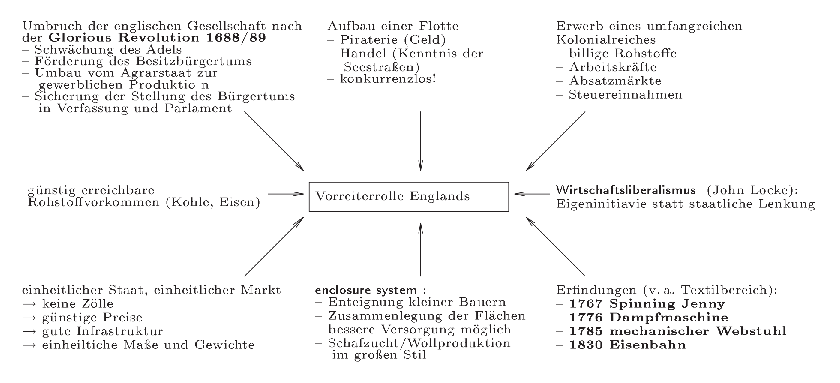
\includegraphics[width=\textwidth]{vorr-gb-gr.eps}
\caption{Ursachen für die Vorreiterrolle Englands}
\label{pic:vorr-gb-gr}
\end{figure}

\endinput
